% !TeX root = ../report-smc.tex
% !TeX encoding = UTF-8
% !TeX spellcheck = en_GB

\section*{PRISM Tutorial Part 3: Dynamic power management}

  \subsection*{Dynamic power management}

    In Section will be described the modelization through PRISM of a \textit{DPM} (\textit{Dynamic Power Management}) system, following the PRISM tutorial found at \cite{prism-tutorial3}. DPMs are used to apply different power usages to some computing device, according to a predefined strategy that takes into account the current state of the device. This kind of systems have been studied largely in literature, for example in \cite{qiu2001stochastic} where a DPM for a Fujitsu disk drive has been studied.
    
    A generic DPM system is made of three distinct components:
    
    \begin{itemize}
      \item \textit{Service Queue} (\textit{SQ}): holds the requests that the Service Provider will have to serve, in an ordered fashion, and can have finite queue capacity;
      \item \textit{Service Provider} (\textit{SP}): serves, one at a time, the requests stored in the Service Queue, serving each time the request at the head of the queue;
      \item \textit{Power Manager} (\textit{PM}): can change the power state of the Service Provider according to certain policies.
    \end{itemize}
    
    The \textit{SP} could be anything that is a computing device that serves requests, such as a disk drive as in \cite{qiu2001stochastic}, but also a CPU or a Web Server.
    
    At any given time, the \textit{SP} is in one of three possible power states, each of which:
    
    \begin{itemize}
      \item \textit{sleep}: the \textit{SP} is in a low-power consumption mode and is unable to serve any request unless explicitly awaken by the \textit{PM};
      \item \textit{idle}: the \textit{SP} is awake but currently not serving any request, so any newly arriving request will be served immediately by the \textit{SP};
      \item \textit{busy}: the \textit{SP} is currently serving a request and will be available to serve the next in queue as soon as it's finished.
    \end{itemize}
    
    Ideally, when in the \textit{sleep} state the \textit{SP} will be requiring little to none power, when in the \textit{idle} state it will require more, as it is awake and ready to serve requests, while when \textit{busy} it will require even more, as the \textit{SP} in that case is actively working on a request. The \textit{PM} is charged with employing a power consumption strategy by switching the \textit{SP}'s power state, in order to maximise the availability of the service while minimising the overall power consumption.
    
    A first PRISM model for a DPM based on \cite{qiu2001stochastic} is proposed in Code \ref{lst:power}, as seen in \cite{prism-tutorial3}.
    
    \begin{center}
      \lstinputlisting[language=prism, caption={PRISM code for the model of a DPM based on \cite{qiu2001stochastic}, with only the \textit{SQ} and the \textit{SP} components. Source \cite{prism-tutorial3}.}, label={lst:power}]{code/power.sm}
    \end{center}
    
    In this first model version shown in Code \ref{lst:power}, only the two modules, for the \textit{SQ} and the \textit{SP} components, are introduced. This is an already working strategy, even without the \textit{PM} component, which would only add a smarter policy for the \textit{SP}'s power management.
    
    It is worth noticing that the model shown in Code \ref{lst:power} is described as a \textit{Continuous Time Markov Chain} (\textit{CTMC}), which allows the use of rates when defining the firing of transitions instead of simple probabilities.
    
    \question{Read the section on \href{http://www.prismmodelchecker.org/manual/ThePRISMLanguage/Synchronisation}{synchronisation} in the manual. Then, have a look at the definition of the \prism{SQ} and \prism{SP} modules, and try to understand what they describe.}
    \answer{
      The \prism{SQ} and \prism{SP} modules implement, respectively, the \textit{SQ} and \textit{SP} components of the DPM system. Both modules synchronise on three different kinds of actions: \prism{request}, indicating the arrival of a new request, \prism{serve}, indicating that a request (except the last) has been served, and \prism{serve_last}, indicating that the last request in the queue has been served.
      
      The \prism{SQ} module keeps a variable, \prism{q}, that represents the current number of request in the queue, with maximum capacity given by the constant \prism{q_max}. When, with the predefined arrival rate \prism{rate_arrive}, a new request arrives (line 26) the queue is updated accordingly, eventually discarding requests in excess in case of a full queue. When a request is served by the \prism{SP} module, whether it was the last (line 30) or not (line 28), the queue is decreased accordingly. The distinction for these two cases might seem useless on the \prism{SQ} side, but it will prove useful for the \prism{SP} module.
      
      The \prism{SP} module only keeps a variable, \prism{sp}, indicating the current power state (0 meaning \textit{sleep}, 1 \textit{idle} and 2 \textit{busy}), which starts in the \textit{idle} state. When a new request arrives, the \textit{SP} is switched to the \textit{busy} state in case it was \textit{idle} (line 51), indicating that it started working on that request right away, while if the power state is either \textit{sleep} or \textit{busy} then it's kept the same (line 54). When a request that was not the last in the queue is served (line 52), with service rate defined by the variable \prism{rate_serve}, the \textit{SP} is kept in the busy state, meaning that it starts working on the next request in line. Otherwise, if the last request is served (line 58), employing the same service rate, the \textit{SP} is switched back to the \textit{idle} state.
      
      It is worth noticing that, since by definition only the \textit{PM} component can decide when the \textit{SP} has to wake, in this first model, if the \textit{SP} starts in the \textit{sleep} state, it would have no way of awaking.
    }
    
    \question{Download the model file \bash{power.sm} from above and load it into PRISM.\\}
    \answer{
      The model \bash{power.sm} loaded into PRISM is shown in Figure \ref{fig:loaded_model}.
    	\begin{figure}[h!]
    		\begin{center}
    			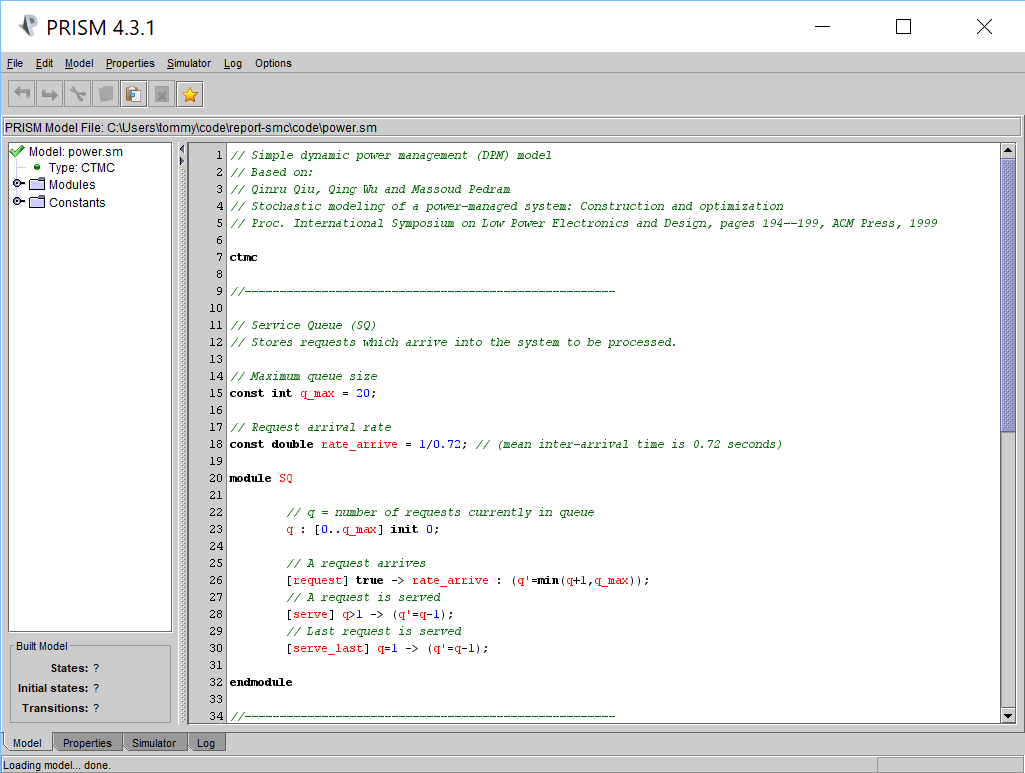
\includegraphics[scale=0.8]{loaded_model.png}
    		\end{center}
    		\caption{Model power.sm loaded into PRISM.}
    		\label{fig:loaded_model}
    	\end{figure}
    }
    
    \question{Use the PRISM simulator to generate some random paths through the model. Notice how, for a CTMC model like this, the elapsed time as the path progresses is displayed in the table. You will probably find that the size of the queue (\prism{q}) never gets above 1. Why is this? Generate a path by hand where the queue reaches its maximum size (currently \prism{q_max}=20). What happens when more requests arrive while the queue is full?}
    \answer{
      By repeatedly selecting the ``Simulate'' button in the PRISM simulator with 1 step it can effectively be seen that the queue size almost never exceeds 1. This because of how arrival and service rates are defined: while the arrival rate of new requests is $1.3\overline{8}$, meaning that on average a new request arrives every $0.72$ seconds, the service rate is $125$, meaning that on average a request is served in $0.008$ seconds. This means that, when a request is in the queue, the service time of that request is, on average, $90$ times faster than the arrival of a new request. So, although possible, it's just highly unlikely that, with rates so defined, a new request arrives before a service is finished.
      
      If instead the action \prism{request} is repeatedly selected in the PRISM simulator in order to force the arrival of new requests before the service, a full queue can be reached. In this case, as expected, more request arrivals end up in the refusal of these new requests, simply no including them in the queue, which remains at it's full capacity (\prism{q_max}=20 in this case). It is worth noticing that, in case a new request arrives before a service is completed, even though the \prism{serve} action remains enabled, it's probability distribution remains the same, since these are all exponentially distributed transitions and thus memoryless.
    }
    
    \question{What is the size of the state space of this model? (i.e from the initial state, how many possible different states can be reached?) Go back to the ``Model'' tab of the GUI, select menu option ``Model | Build model'' and then look at the statistics displayed in the bottom left corner to check your answer.}
    \answer{
      By selecting the ``Build model'' feature, it can be seen that the state space of this model is made of a total of 21 states. Intuitively, these are made of a state where the \textit{SP} is \textit{idle} and the queue empty and 20 states where the \textit{SP} is \textit{busy} and the queue has a different number of pending requests (from 1 to 20).
    }
    
  \subsection*{Adding the power management control}
  
    Now we add to the PRISM model shown in Code \ref{lst:power} and additional module, \prism{PM}, responsible of implementing the Power Manager. The \textit{PM} is the component of a DPM that is charged with waking the \textit{SP} from sleep or putting it back to sleep according to a specific policy that might be dependent of several factors, such as the current state of the \textit{SP} or of the \textit{SQ}.
    
    Code \ref{lst:power_policy1} shows the updated model with the added \prism{PM} module, which employs a fairly naive policy.
    
    \begin{center}
      \lstinputlisting[language=prism, caption={PRISM code for the model of a DPM based on \cite{qiu2001stochastic}, with the \textit{SQ}, \textit{SP} and \textit{PM} components. Source \cite{prism-tutorial3}.}, label={lst:power_policy1}]{code/power_policy1.sm}
    \end{center}
    
    \question{Look at the code we have added to the \prism{SP} module and at the new \prism{PM} module. Make sure you understand how they work.}
    \answer{
      
    }
